\chapter{Implementation}

In this chapter, the process of implementation will be covered, starting by the architecture and the tools to the results and how everything fits together.

\section{Tools}
\subsection{React JS}

\begin{wrapfigure}[10]{r}{3cm}
	\vspace{-10pt}
	
\includegraphics[width=3cm]{images/chapter3/logo-react-js.png}
	\vspace{-10pt}
	\caption{{\footnotesize React JS framework logo}}
\end{wrapfigure}

React (also known as React.js or ReactJS) is a free and open-source front-end JavaScript library\cite{ReactJavaScriptLibrary} for building user interfaces or UI components. It is maintained by Facebook and a community of individual developers and companies.\cite{ReactMakingFaster} React can be used as a base in the development of single-page or mobile applications. However, React is only concerned with state management and rendering that state to the DOM, so creating React applications usually requires the use of additional libraries for routing, as well as certain client-side functionality.

\subsection{Web3.js}

There are a few different aspects to developing blockchain applications with Ethereum:

\begin{itemize}
\item \textbf{Smart contract development} - writing code that gets deployed to the blockchain with the Solidity programming language.
\item \textbf{Developing websites or clients that interact with the blockchain} - writing code that reads and writes data from the blockchain with smart contracts.
\end{itemize}

\begin{wrapfigure}[9]{r}{3cm}
	\vspace{-10pt}
	
\includegraphics[width=3cm]{images/chapter3/web3.jpeg}
	\vspace{-10pt}
	\caption{{\footnotesize Web3 logo}}
\end{wrapfigure}

Web3.js enables you to fulfill the second responsibility: developing clients that interact with The Etherem Blockchain. It is a collection of libraries that allow you to perform actions like sending Ether from one account to another, read and write data from smart contracts, create smart contracts, and so much more.

Web3.js communicates to The Ethereum Blockchain with JSON RPC, which stands for "Remote Procedure Call" protocol. Ethereum is a peer-to-peer network of nodes that stores a copy of all the data and code on the blockchain. Web3.js allows us to make requests to an individual Ethereum node with JSON RPC in order to read and write data to the network\cite{mccubbinIntroWeb3Js}.

\subsection{Ganache}

\begin{wrapfigure}[11]{r}{2.5cm}
	\vspace{-10pt}
	
\includegraphics[width=2.5cm]{images/chapter3/ganache-logo-dark.png}
	\vspace{-10pt}
	\caption{{\footnotesize Ganache Logo}}
\end{wrapfigure}

Ganache is a personal blockchain for rapid Ethereum and Corda distributed application development. You can use Ganache across the entire development cycle; enabling you to develop, deploy, and test your dApps in a safe and deterministic environment.

Ganache comes in two flavors: a UI and CLI. Ganache UI is a desktop application supporting both Ethereum and Corda technology. The command-line tool, ganache-cli (formerly known as the TestRPC), is available for Ethereum development. Prefer using the command-line? This documentation will focus only on the UI flavor of Ganache. Please see the Ganache CLI Readme for command-line documentation.

All versions of Ganache are available for Windows, Mac, and Linux\cite{GanacheOverviewDocumentation}.

\begin{figure}[H]
	\centering
		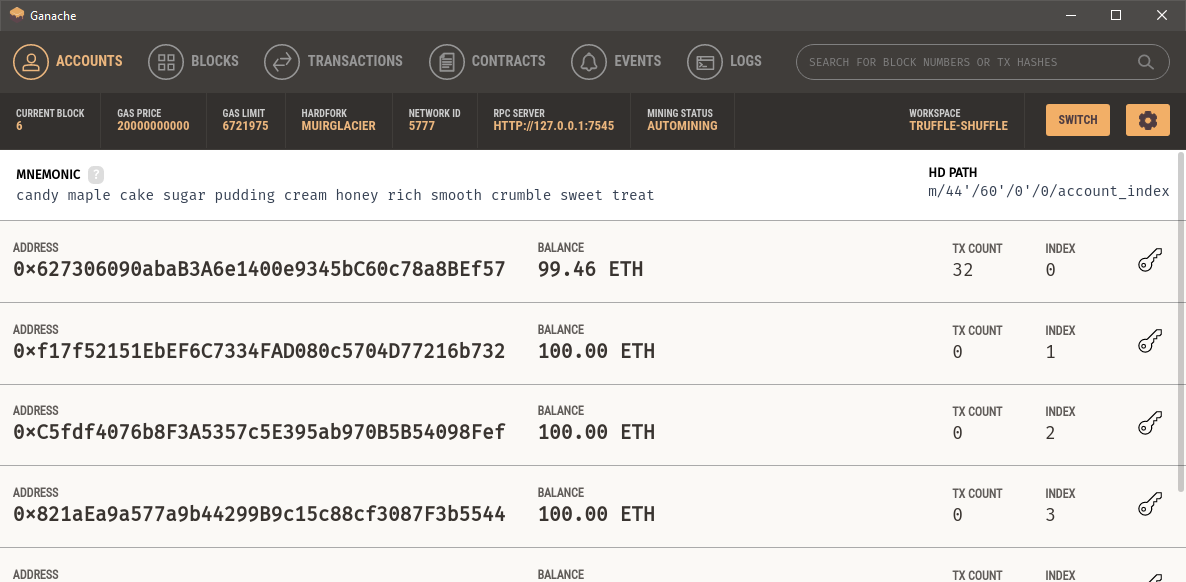
\includegraphics[width=10cm]{images/chapter3/ganache-window.png}
		\caption{{\footnotesize Ganache GUI}}
\end{figure}

\subsection{MetaMask}

\begin{wrapfigure}[10]{r}{2.5cm}
	\vspace{-10pt}
	
\includegraphics[width=2.5cm]{images/chapter3/metamask-logo.png}
	\vspace{-10pt}
	\caption{{\footnotesize MetaMask Logo}}
\end{wrapfigure}

MetaMask is a software cryptocurrency wallet used to interact with the Ethereum blockchain.\cite{schroederCryptoWalletMetaMask2020} It allows users to access their Ethereum wallet through a browser extension or mobile app, which can then be used to interact with decentralized applications.

MetaMask allows users to store and manage account keys, broadcast transactions, send and receive Ethereum-based cryptocurrencies and tokens, and securely connect to decentralized applications through a compatible web browser or the mobile app's built-in browser.[3][4]

The application includes an integrated service for exchanging Ethereum tokens by aggregating several decentralized exchanges (DEXs) to find the best exchange rate. This feature, branded as MetaMask Swaps, charges a service fee of 0.875\% of the transaction amount\cite{schroederCryptoWalletMetaMask2021}.

\begin{figure}[h]
	\centering
		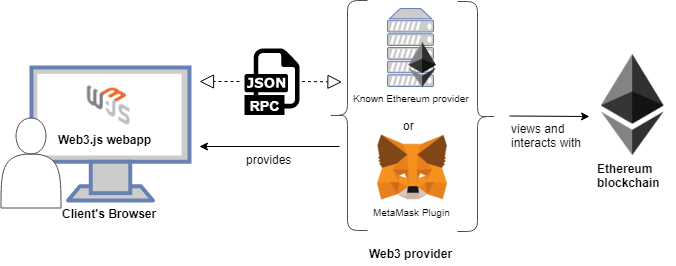
\includegraphics[width=12cm]{images/chapter3/web3-architecture.png}
		\caption{{\footnotesize the architecture of a client application interaction with a blockchain network using Web3 and MetaMask}}
\end{figure}

\section{System Design}

In this section, we introduce our proposed voting system that aims to solve some of the barriers that traditional voting systems have.

\subsection{Architecture}

\begin{figure}[H]
	\centering
		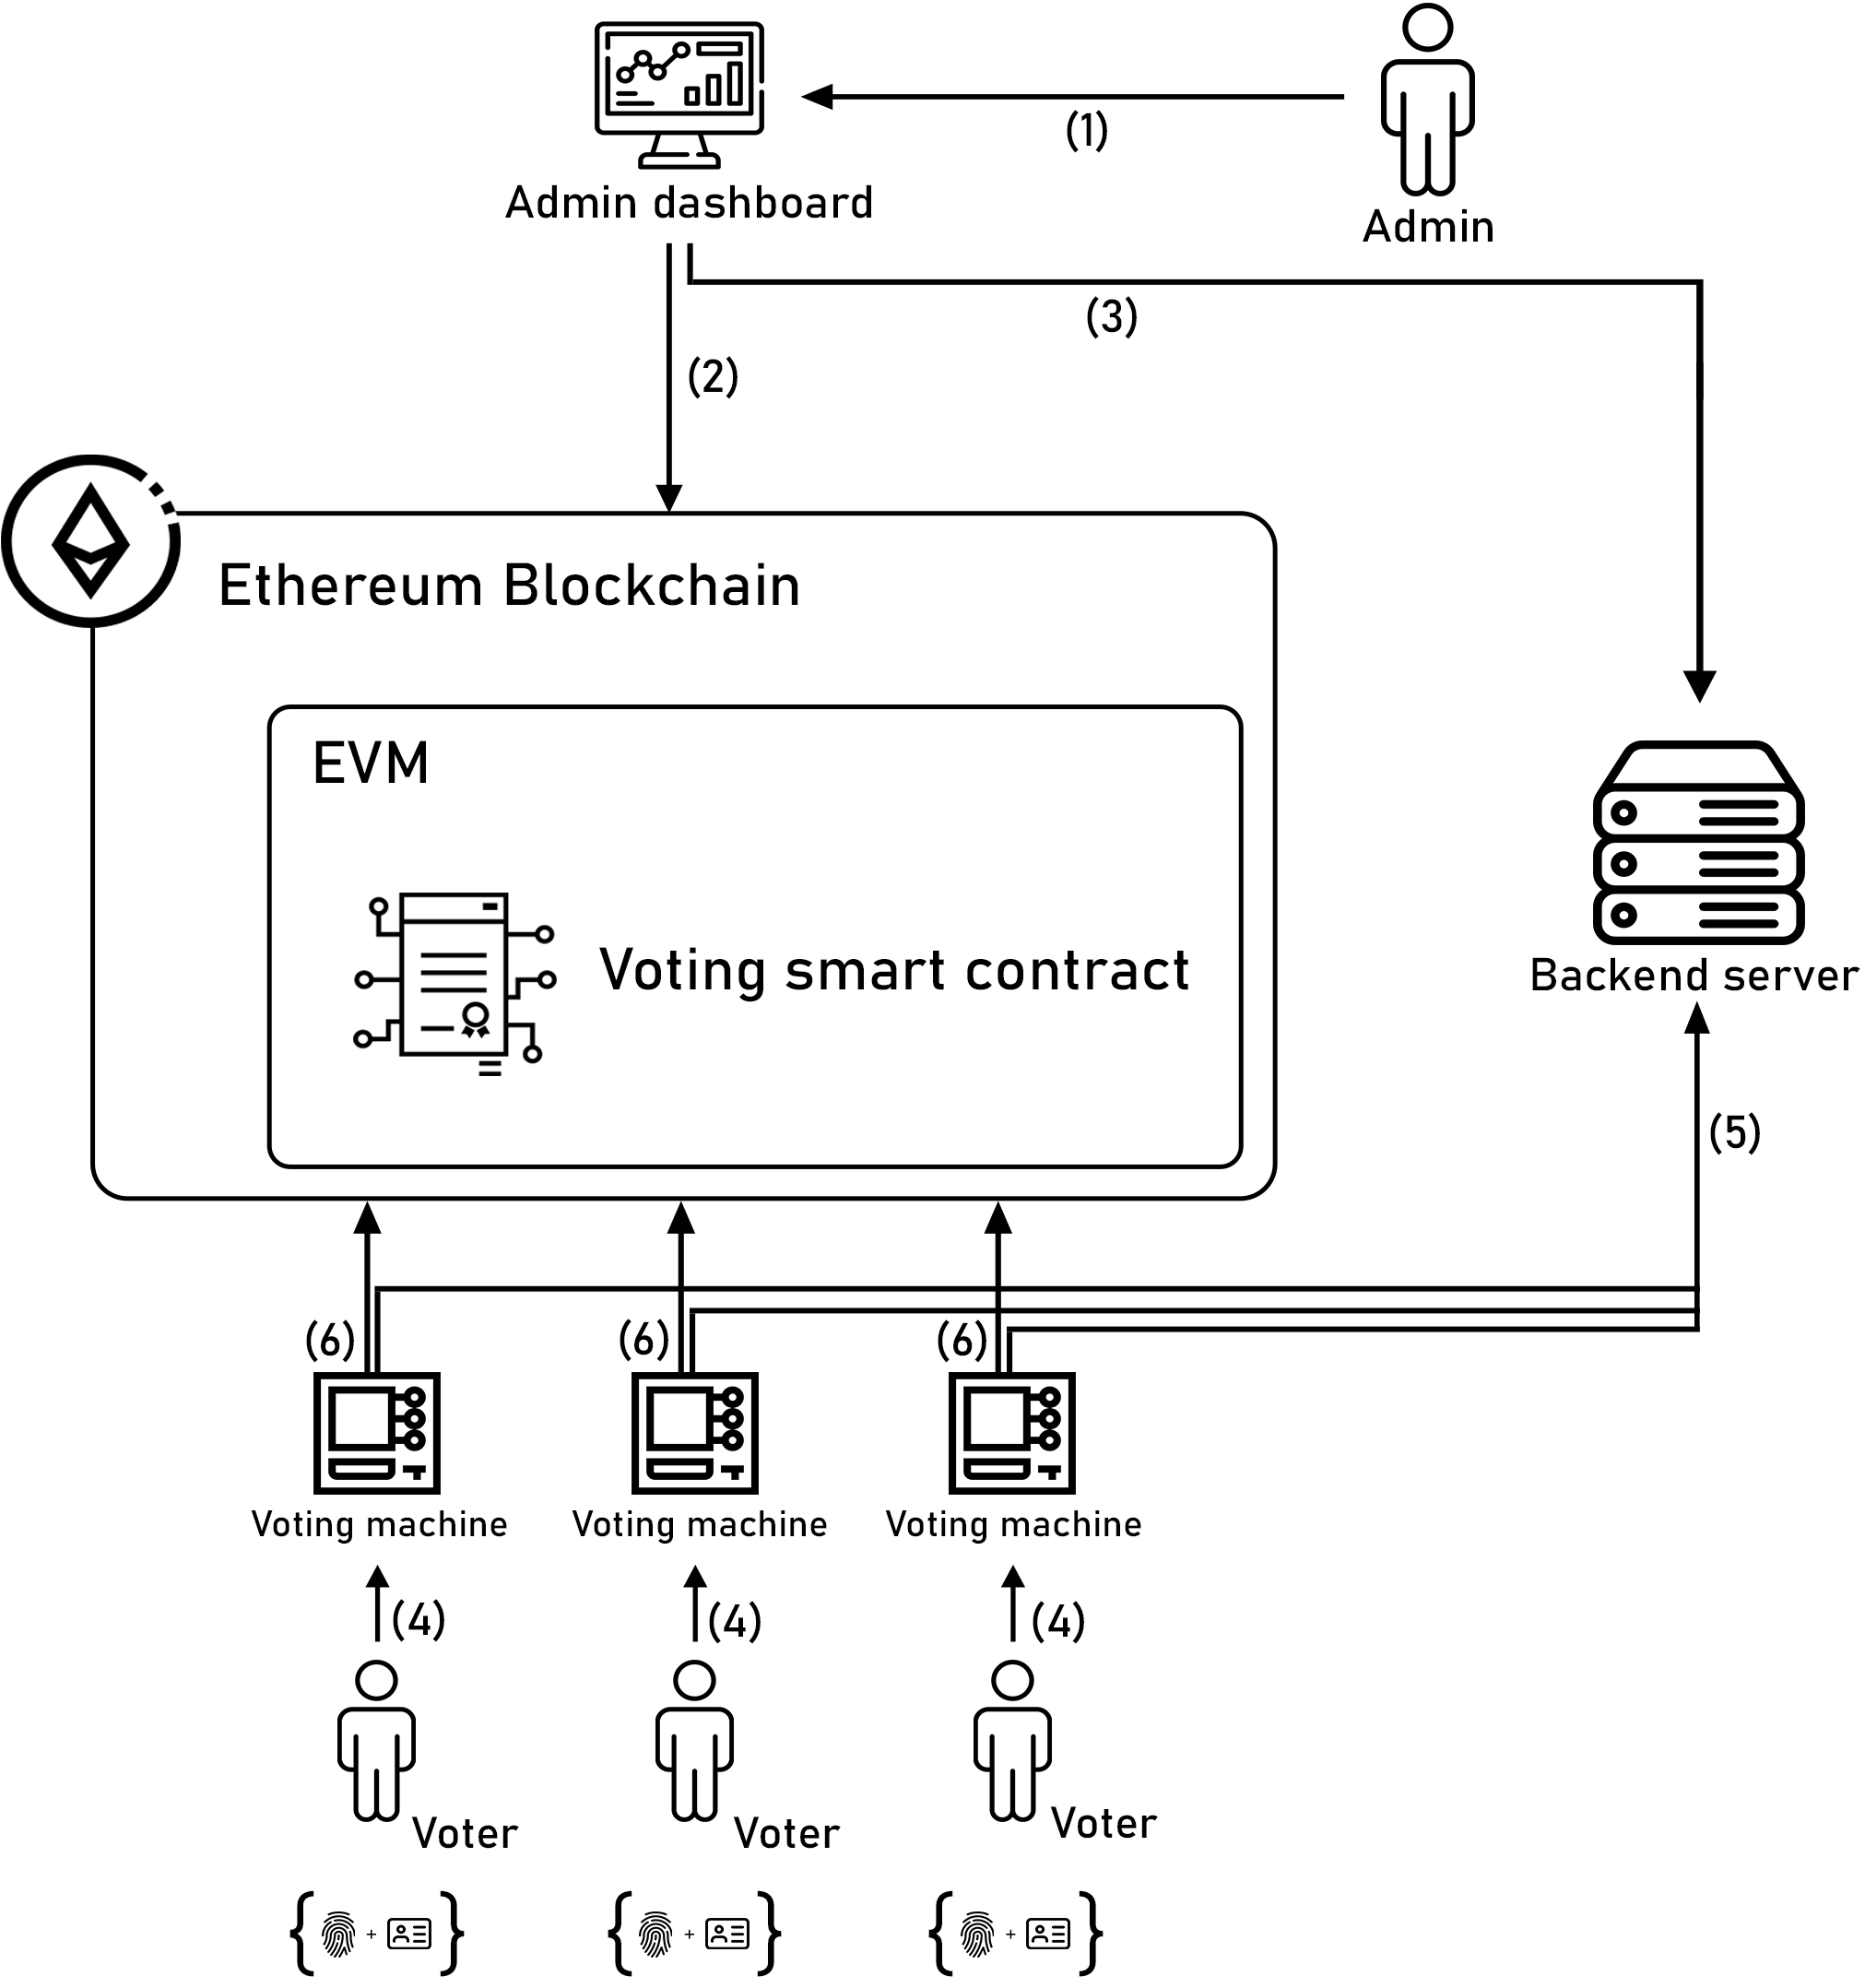
\includegraphics[width=12cm]{images/chapter3/architecture.png}
		\caption{{\footnotesize High level architecture of the proposed system and the interaction between its components}}
\end{figure}

\begin{list}{}{}
\item \textbf{(1)} The admin operating the dashboard launches and monitors voting events
\item \textbf{(2)} Essential data (candidates name and id, event title, start \& finish dates) are saved in the blockchain along with the list of authorized accounts that can interact with the smart contract.
\item \textbf{(3)} Secondary data that is of less importance is saved to the regular (centralized) backend server.
\item \textbf{(4)} Voters authenticate themselves to the polling machines (using biometric means) and cast their vote for a candidate of their choosing
\item \textbf{(5)} Voting machines use the backend server to verify the identity of the voter and to fetch secondary data required for the displaying of candidates
\item \textbf{(6)} Voting machines saves the submitted choice to the blockchain by launching a transaction that increments the vote count of the chosen candidate
\end{list}

\subsection{Diagrams}
\subsubsection{Admin sequence diagram}

\begin{figure}[H]
	\centering
		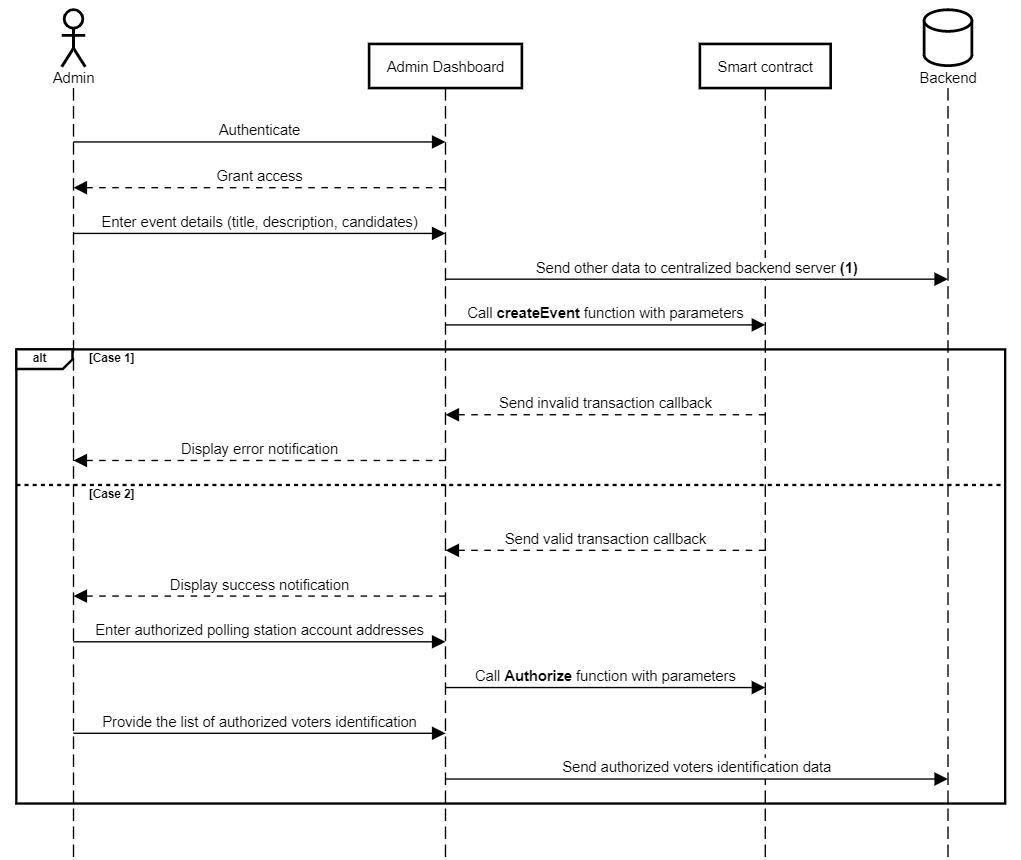
\includegraphics[width=14cm]{images/chapter3/admin_sequence_diagram.png}
		\caption{{\footnotesize Sequence diagram of the process of creating and launching a new voting event}}
\end{figure}

Launching an election requires that the administrator get access to the administration dashboard which has its access restricted by digital or physical boundaries or both, using the dashboard the administrator accesses the event creation form, in which he fills the information for the event. The information provided will be divided on the basis of their level of criticality, for example, candidates' pictures and lengthy descriptions are deemed to be less critical to the vote-counting so they're stored in a regular backend server. Also, information required for the authentication of voters is also stored on the regular backend servers.

Next, the administrator is tasked with providing the account addresses of the ethereum accounts running on each voting machine, this list will be the list of the ethereum account addresses allowed to interact with the smart contract and alter the vote count of any candidates by incrementing it.

\subsubsection{Voter sequence diagram}

\begin{figure}[H]
	\centering
		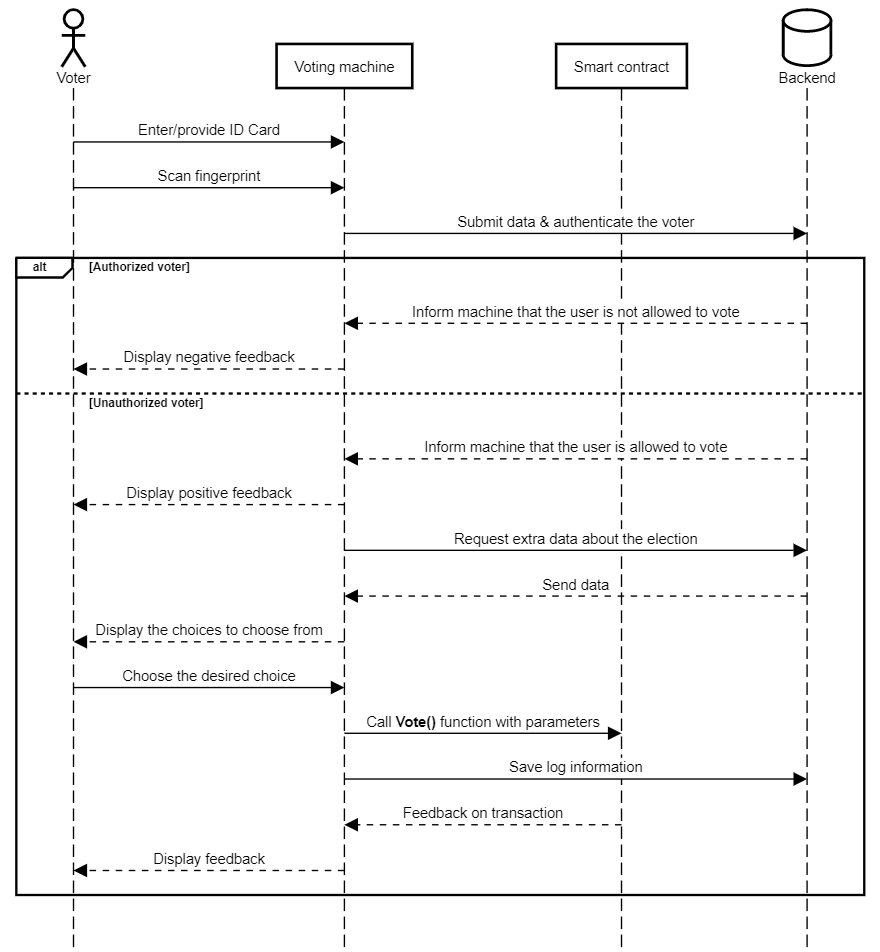
\includegraphics[width=14cm]{images/chapter3/voter_sequence_diagram.png}
		\caption{{\footnotesize Sequence diagram of the process of casting a vote}}
\end{figure}

The process of casting a vote is initiated when a voter first enters a polling station, then proceeds to a vacant voting machine, the machine should be equipped with an ID Card reader and fingerprint scanner to conduct a biometric identity check. the information obtained will be checked against the records saved on the backend server. In case the person is identified as an authorized voter; meeting whatever the requirements listed by the entity organizing the voting event (for example an entity can enforce one single vote per household or set the minimum age for participation to 50), a list of choices will be displayed to the voter to choose from in an intuitive manner after the voter makes his choice and submits it, the voting machine performance an ethereum transaction to the smart contract by calling the appropriate function that will result in incrementing the vote count of that particular candidate, also log information about the vote will be saved to the backend server.

\section{Results}

To validate the proposed system, we implemented various components of the proof-of-concept using various technologies highlighted in previous sections, in this section we will go through the results that were obtained by this investigatory effort.

\subsection{Admin dashboard}

The admin dashboard is a web application developed using React JS framework and the UI components library Shards\cite{ShardsReact}, it serves as the starting point of every election event. The admin is impelled to use this unique platform to create, launch and monitor a voting event.

The access to this platform should be very restricted, as well as the ethereum account associated with it, being conceptualized to be the sole orchestrator of the whole event, this application (and account) has various privileges granted to from the deployed smart contracts, things like creating an event, terminating an event, granting voting authorizations and viewing results.

\begin{figure}[H]
	\centering
		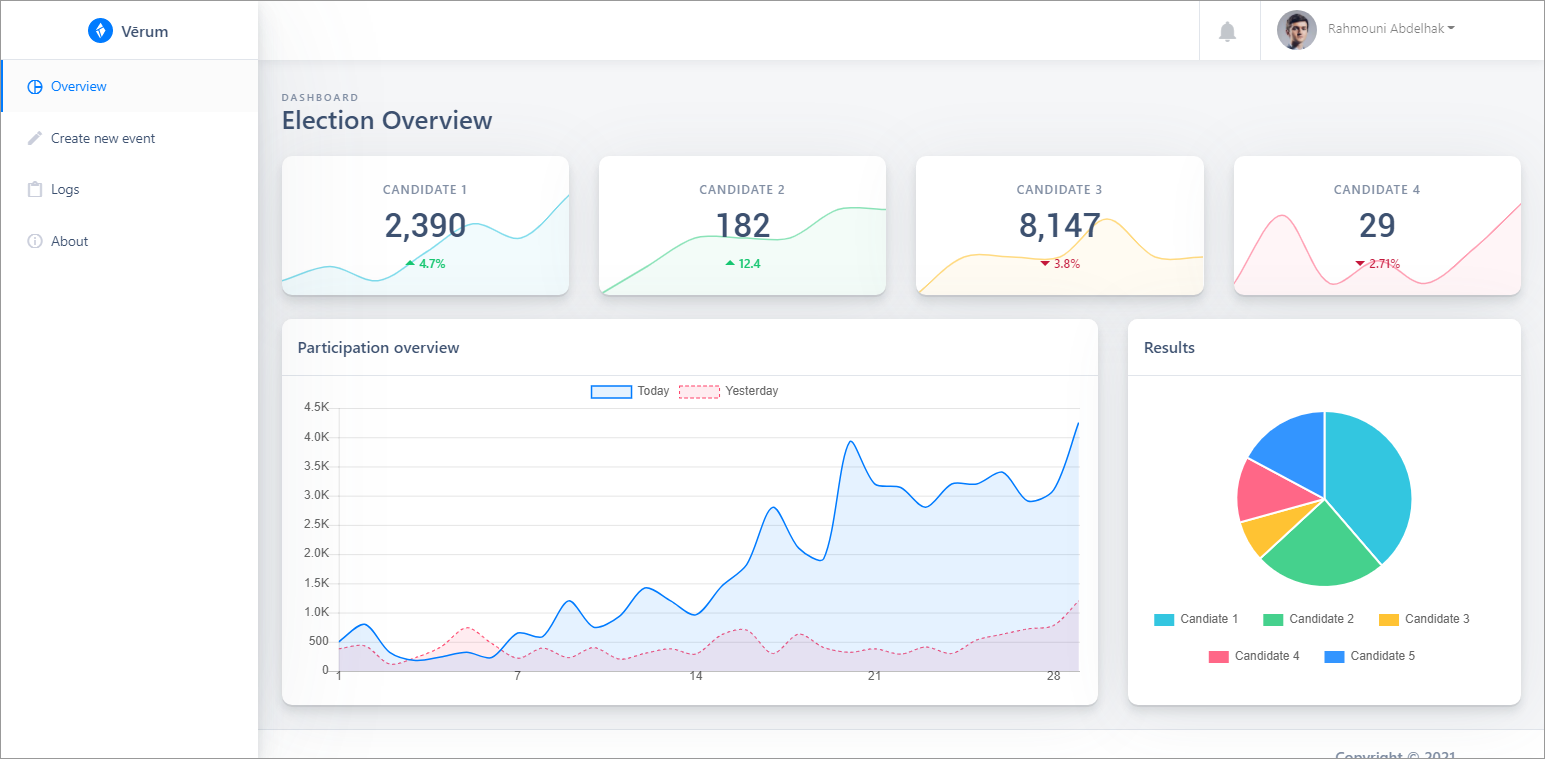
\includegraphics[width=14cm]{images/chapter3/admin_1.png}
		\caption{{\footnotesize Election overview tab of the admin dashboard}}
\end{figure}

The election overview tab is the main tab where the instant monitoring of ongoing election event is done, using various forms of charts and indicators an admin can easily stay up to date with everything occurring on the ongoing event.

\begin{figure}[H]
	\centering
		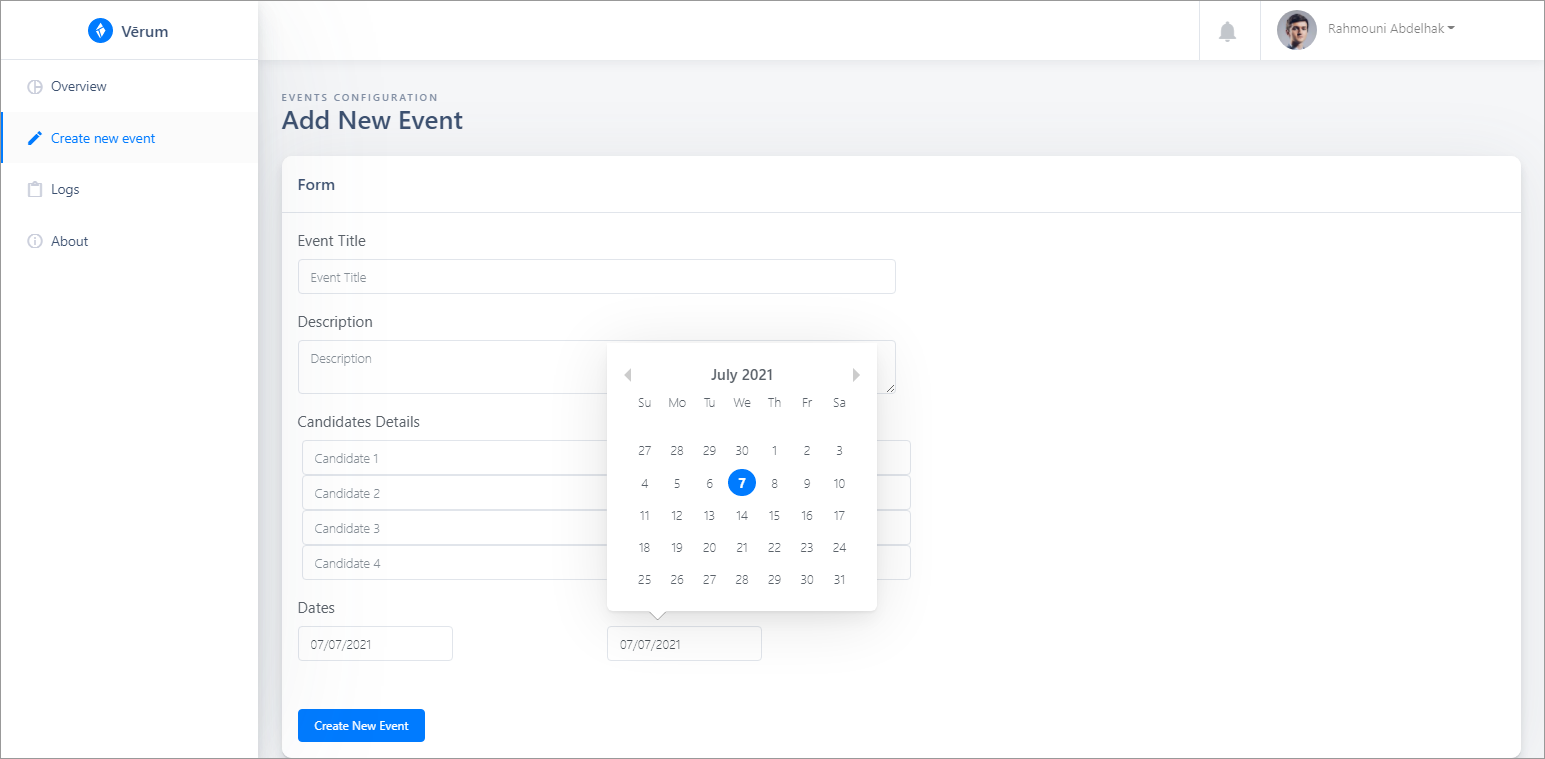
\includegraphics[width=14cm]{images/chapter3/admin_2.png}
		\caption{{\footnotesize Event creation tab of the admin dashboard}}
\end{figure}

Event creation tab holds an event creation form where the admin is provided with inputs fields to fill, information like the event title, description and beginning and end dates along with candidates details are all submitted through this form.

\begin{figure}[H]
	\centering
		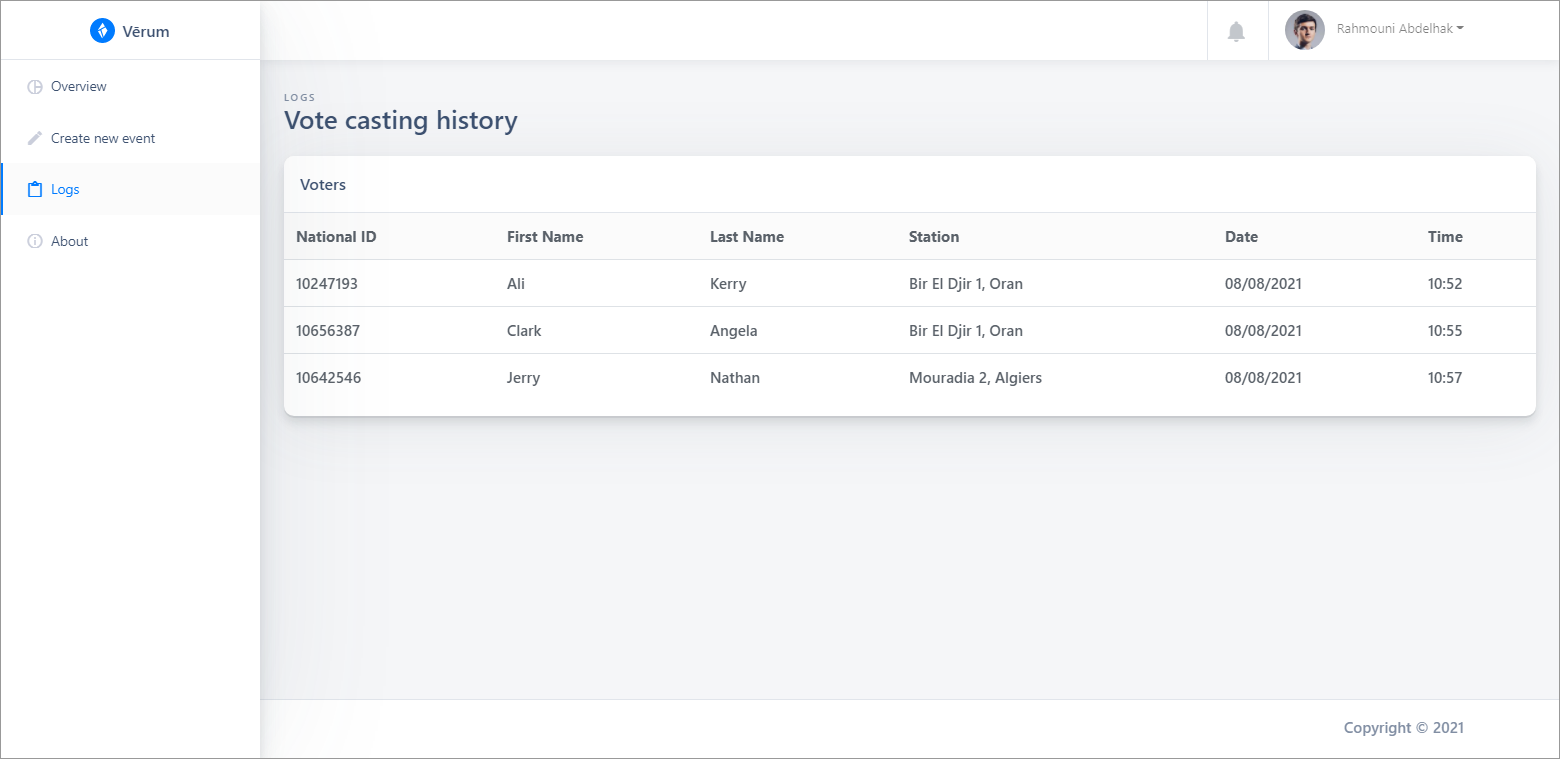
\includegraphics[width=14cm]{images/chapter3/admin_3.png}
		\caption{{\footnotesize Logs tab of the admin dashboard}}
\end{figure}

The logs tab presents a detailed view of the vote casting process history, unlike the election overview tab, this part of the application does not obtain its data from the blockchain ledger, but from the centralized backend that stores the log information of voters separately from the content of their vote.

\subsection{End-user (voter) application}

The voter application lives on the voting machine, although for the sake of our proof-of-concept it was built as a web application, we believe that in a real-world scenario a desktop (native) application with touch screen capabilities would serve the purpose very well.

\begin{figure}[H]
	\centering
		
\includegraphics[width=14cm]{images/chapter3/voter_2.png}
		\caption{{\footnotesize Voter application authentication screen}}
\end{figure}

The voter is first faced with an authentification screen prompting her to provide her national identification number (although in a real-world scenario we would opt for electronic ID scanners) and to also scan her fingerprint, in case the voter is an authorized voter that hasn't, for example, voted before that application allows the user to proceed.

\begin{figure}[H]
	\centering
		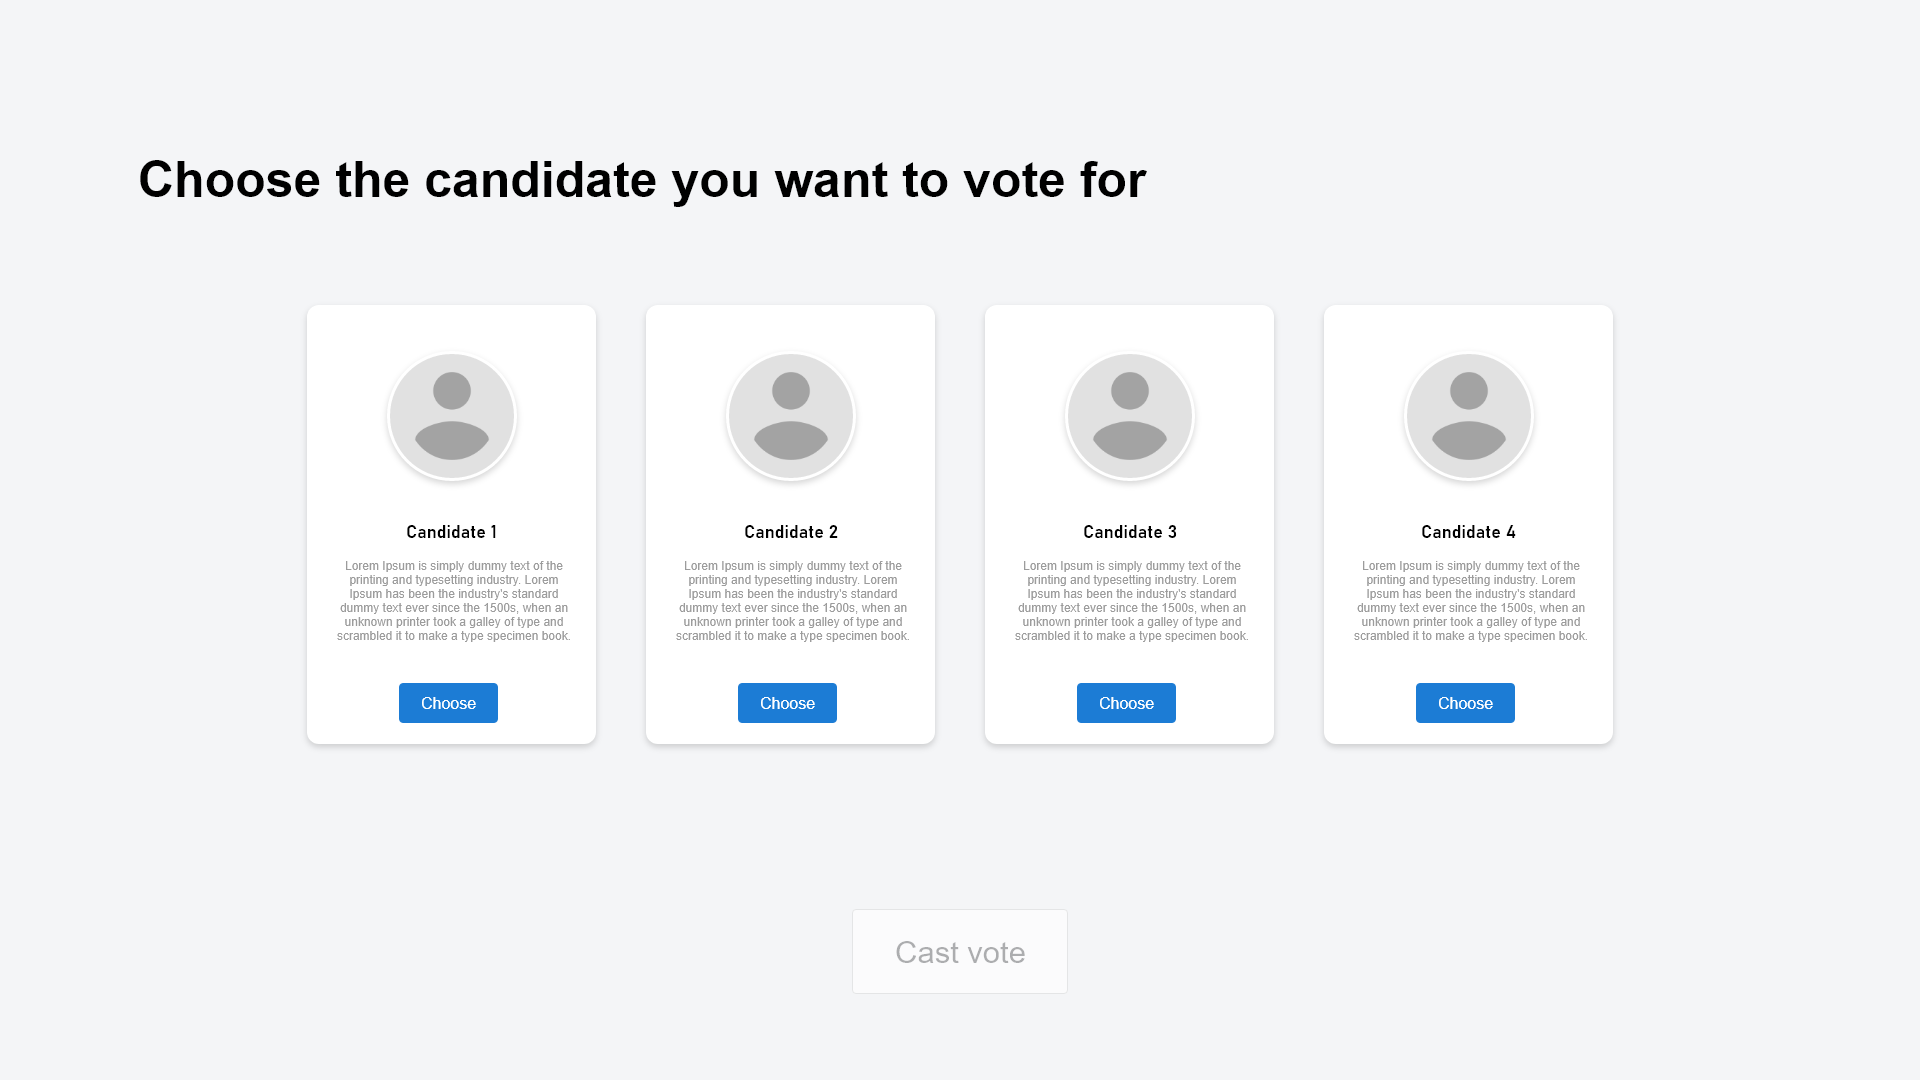
\includegraphics[width=14cm]{images/chapter3/voter_3.png}
		\caption{{\footnotesize Choices presentation screen}}
\end{figure}

Next, the voter is presented with the choices to pick from.

\begin{figure}[H]
	\centering
		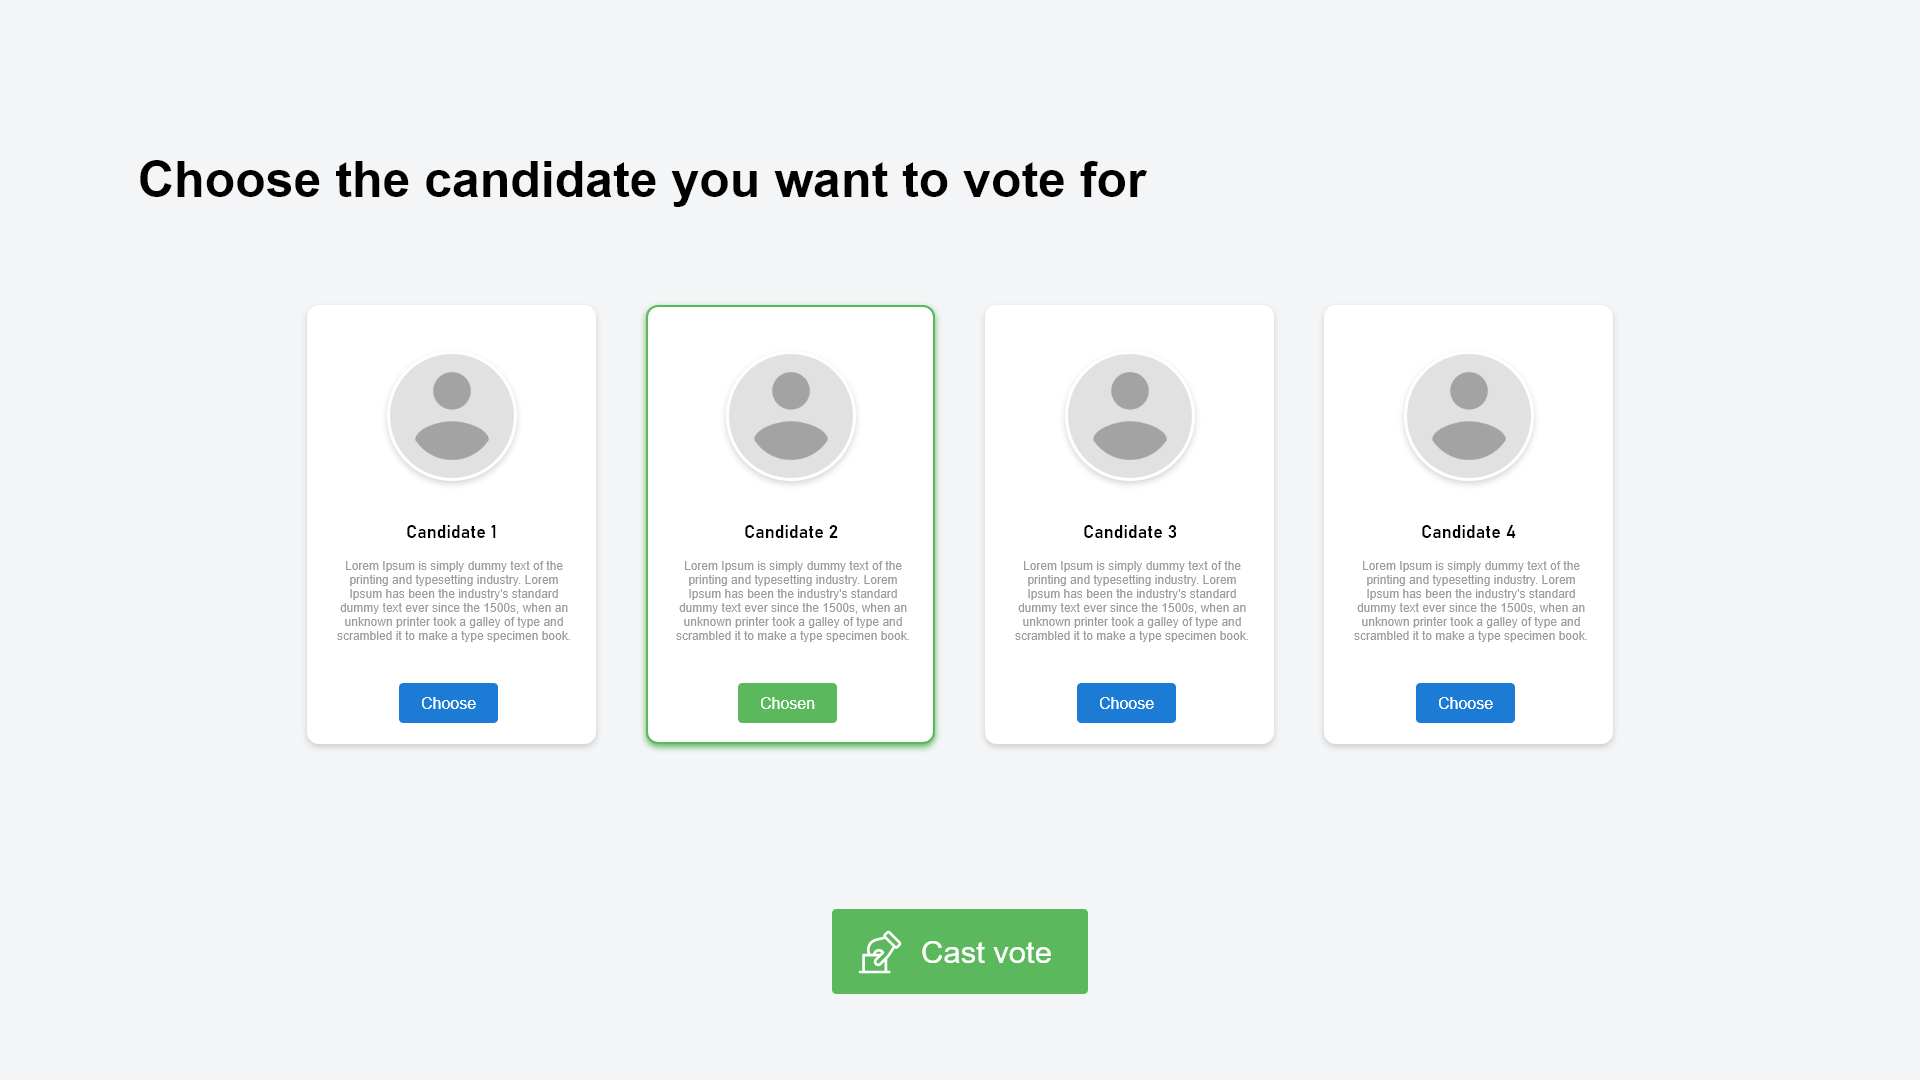
\includegraphics[width=14cm]{images/chapter3/voter_4.png}
		\caption{{\footnotesize Choice submitting screen}}
\end{figure}

After a choice is selected, s submit button is enabled.

\begin{figure}[H]
	\centering
		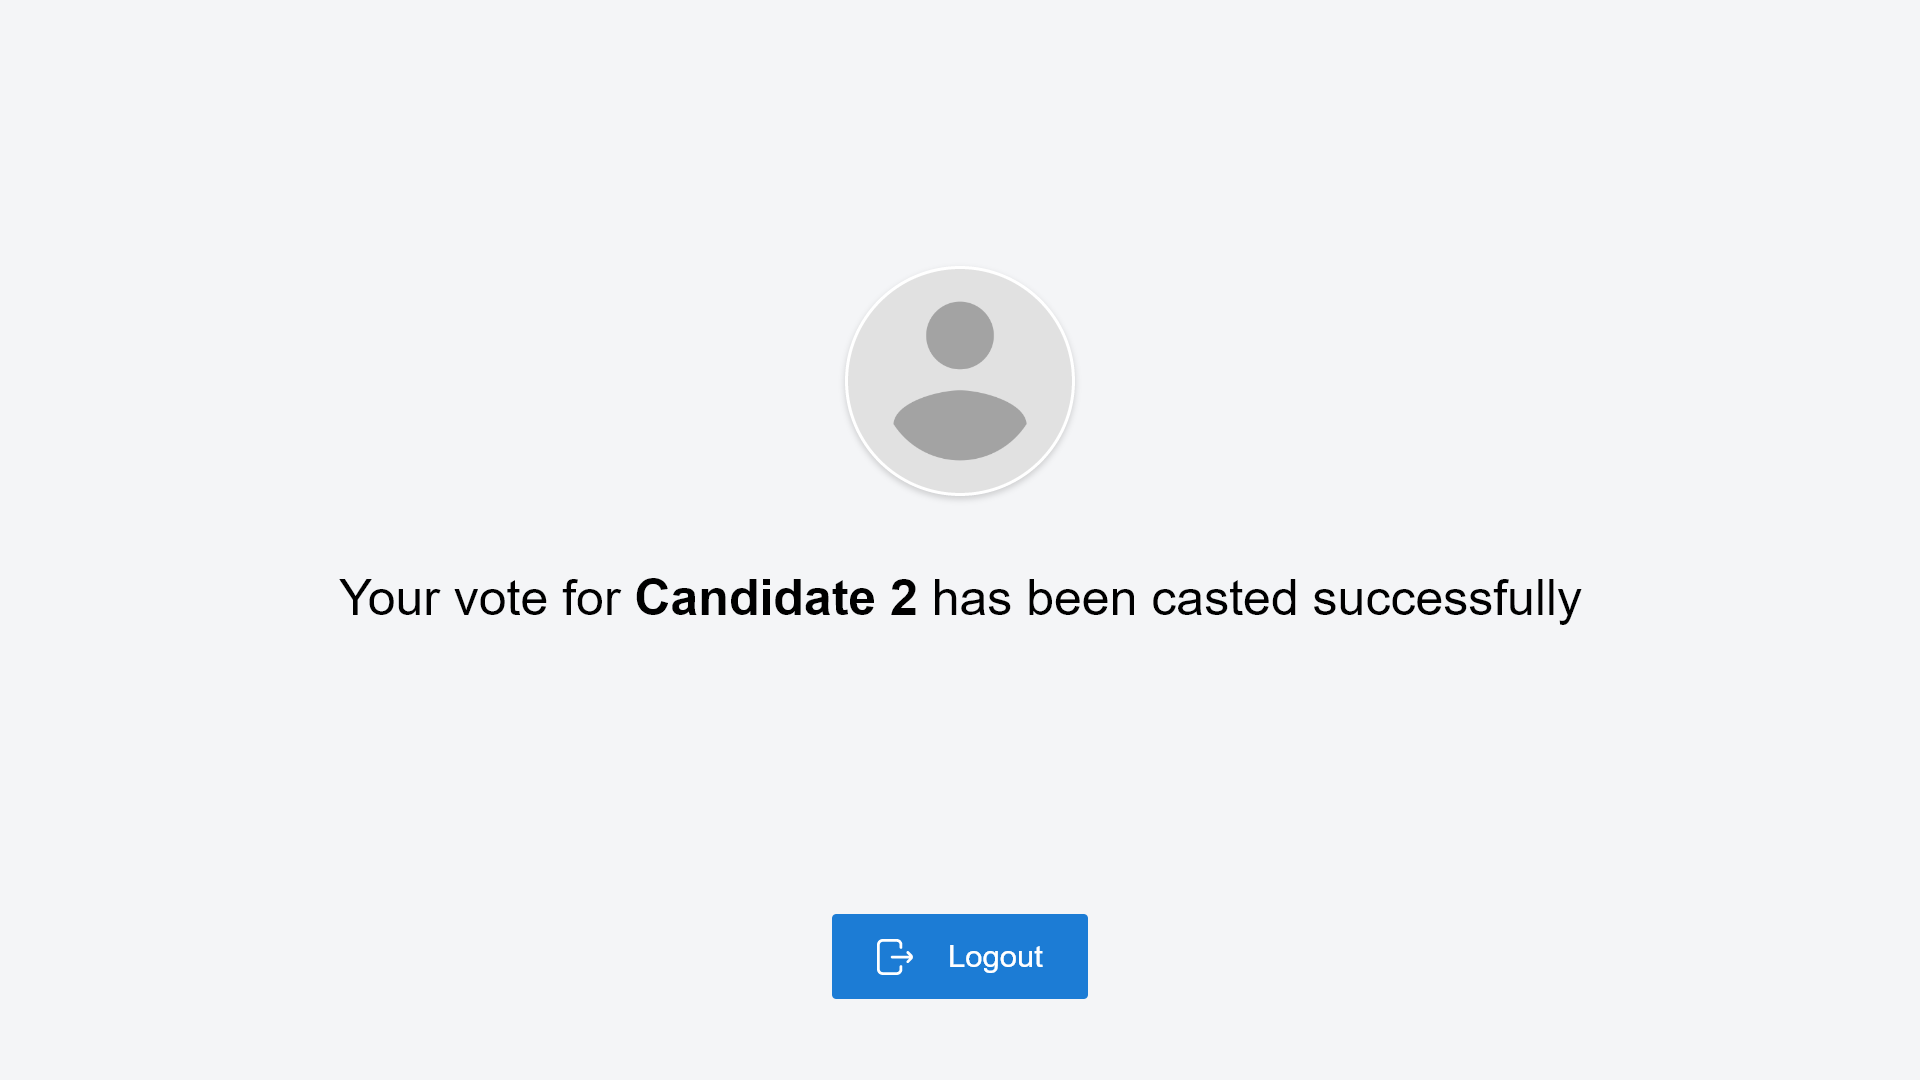
\includegraphics[width=14cm]{images/chapter3/voter_5.png}
		\caption{{\footnotesize Vote casting feedback screen}}
\end{figure}

Lastly, a feedback screen is displayed, then the user is prompted to log out instantly at the end of the voting process or it will log out automatically after a certain amount of time.

\subsection{Smart contract}

\begin{figure}[H]
	\centering
		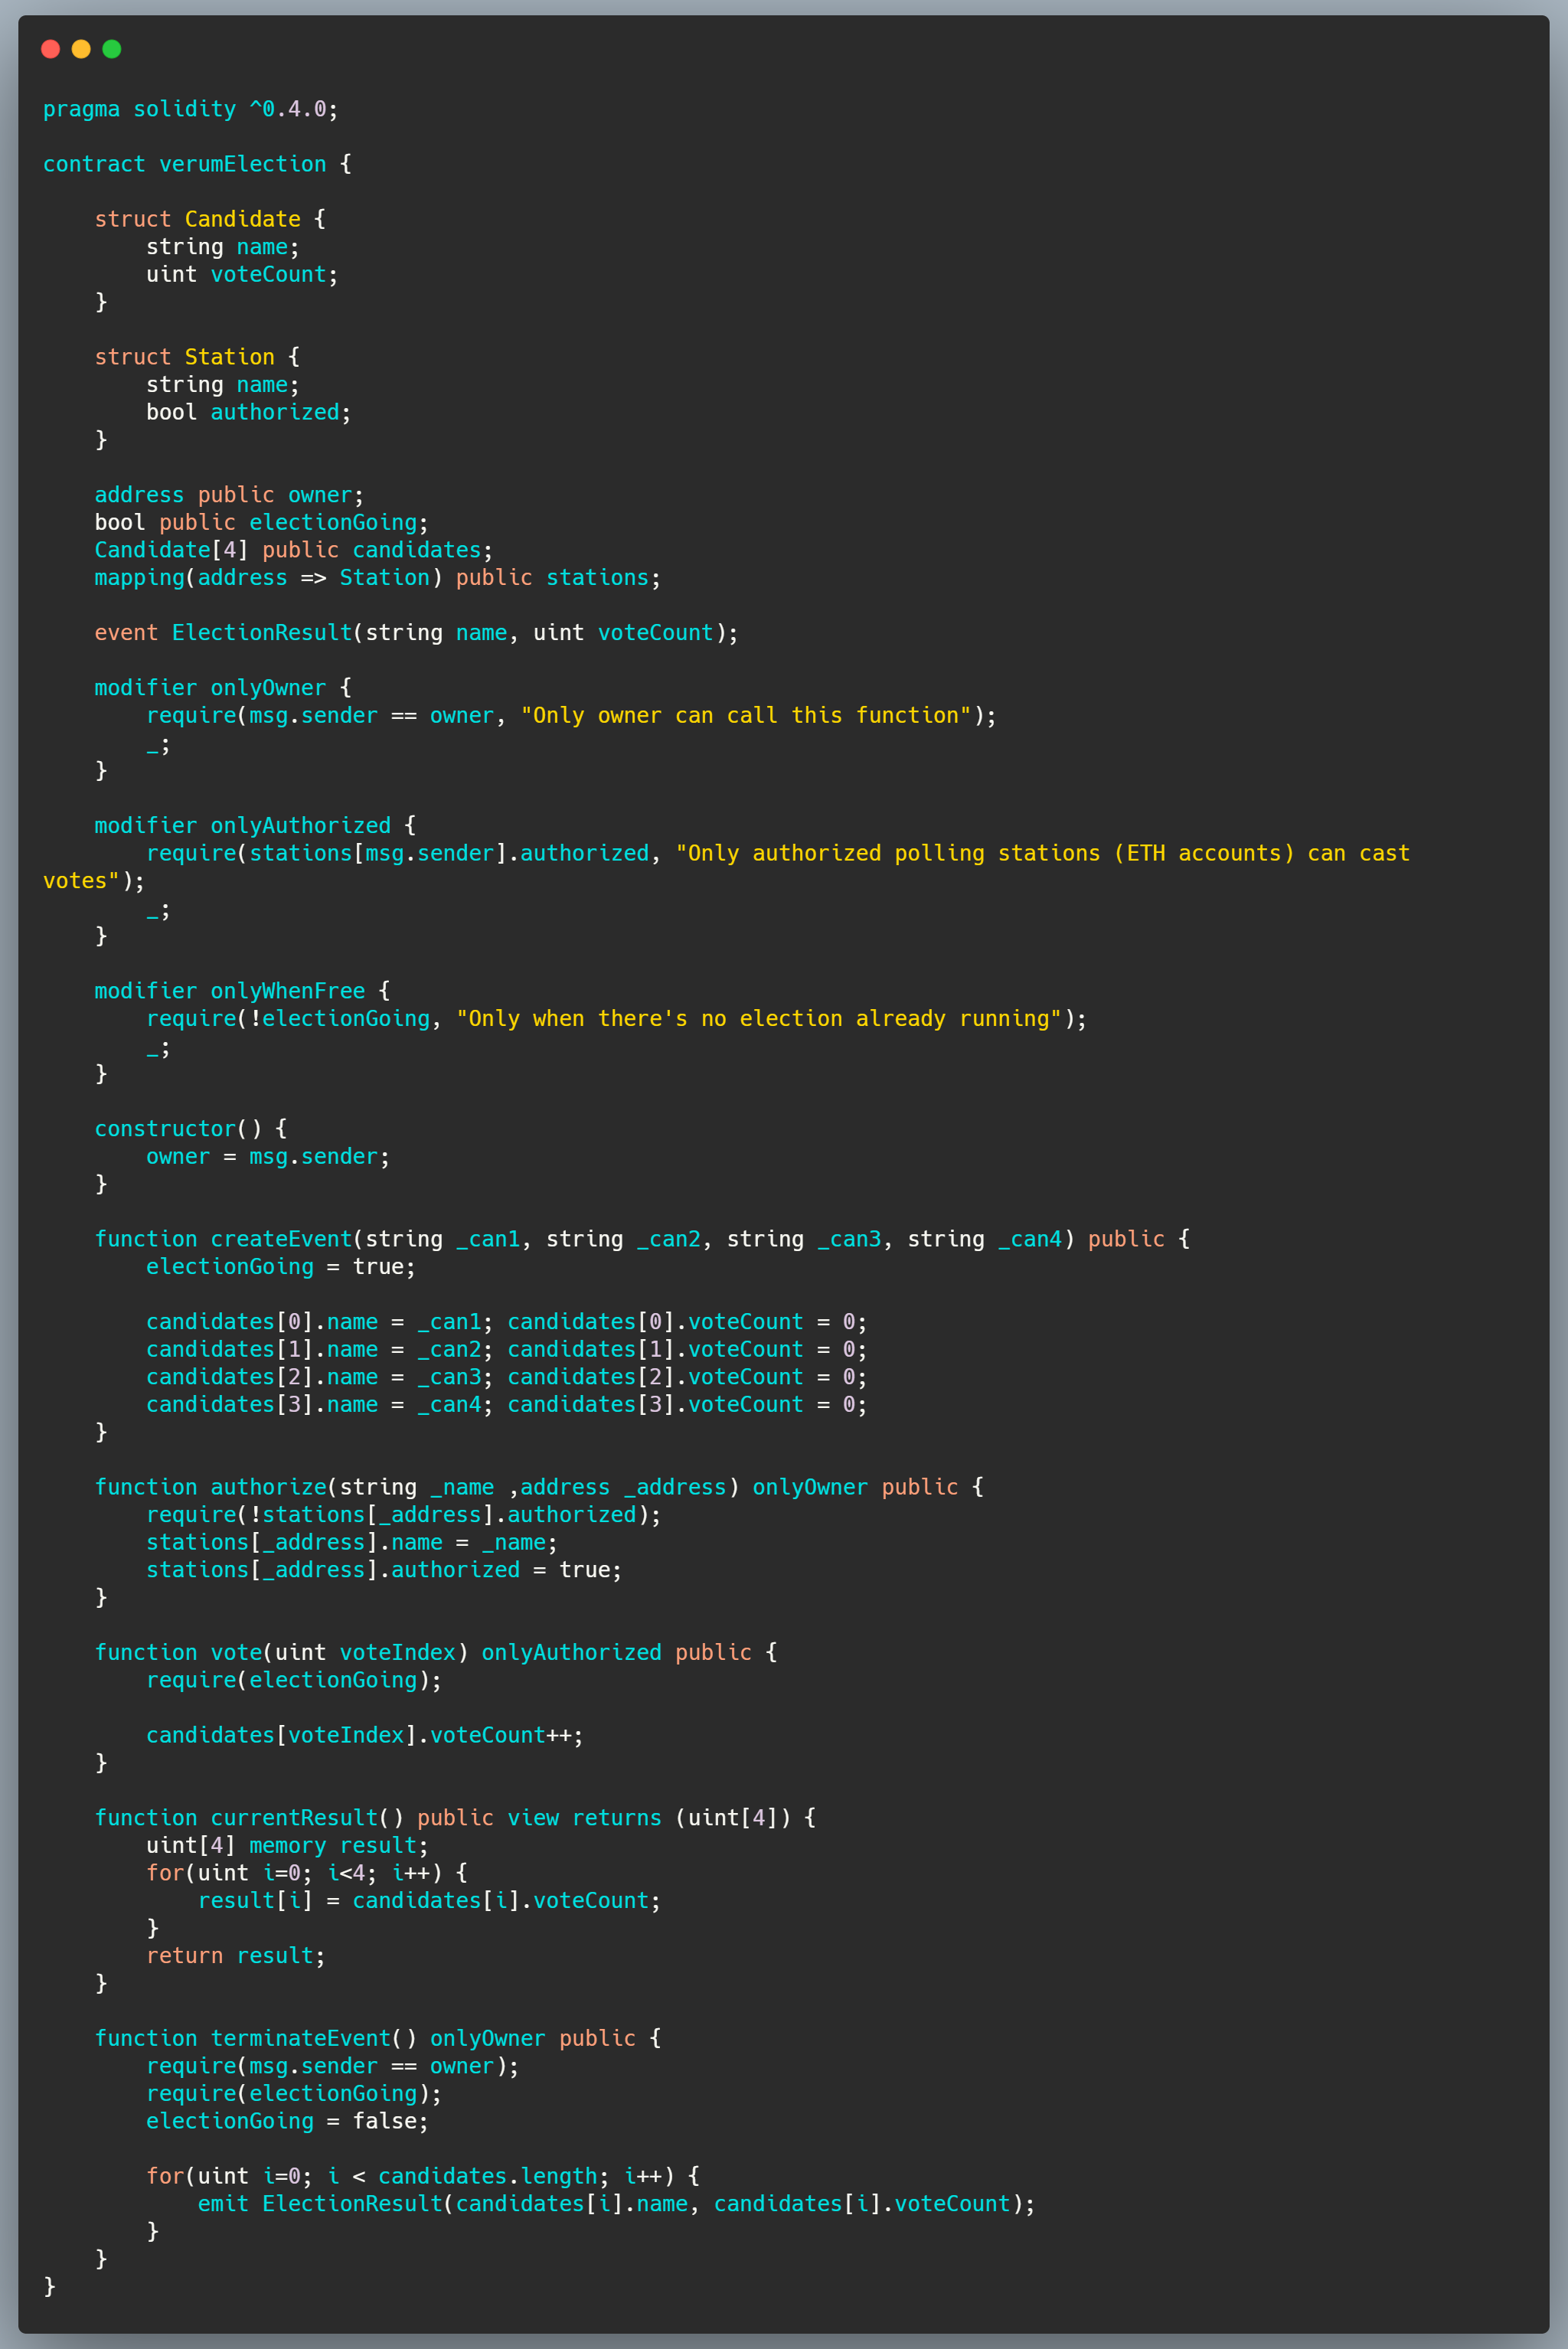
\includegraphics[width=12cm]{images/chapter3/smart-contract.png}
		\caption{{\footnotesize Voting smart contract, written in solidity language}}
		\label{smart_contract}
\end{figure}

The smart contract showed in figure \ref{smart_contract} implements our voting contract.

The idea is to create and deploy a smart contract using the account intended to be of the admin, then using the various functions defined the admin can interact with the smart contract to create a voting event and input information about candidates and whatnot.

\subsubsection{Structres}

Structs are custom defined types that can group several variables

\begin{list}{}{}
\item \textbf{Candidate} is the definition of a struct type representing the information that will stored about a single candidate on the smart contract's state.
\item \textbf{Station} represents the information that will be stored about a single polling station or (a single voting machine, in case each voting machine has a separate ethereum account and address.
\end{list}

\subsubsection{State variables}

State variables are variables whose values are permanently stored in contract storage.

\begin{list}{}{}
\item \textbf{owner} a state variable of type address that holds the addresses of the account that owns the smart contract, being the admin, the holder of that ethereum address has extra privileges when interacting with the smart contract.
\item \textbf{electionGoing} a state variable of type boolean that holds either true when an election event is taking place or false when there's none.
\item \textbf{candidates} an array of the struct type predefined Candidate that holds the list of choices a voter needs to choose from.
\item \textbf{stations} an array of the struct type predefined Station that holds the list of polling stations allowed to cast a vote in this ongoing voting event.
\end{list}

\subsubsection{Event}

Solidity events give an abstraction on top of the EVM’s logging functionality. Applications can subscribe and listen to these events through the RPC interface of an Ethereum client.

\begin{list}{}{}
\item \textbf{ElectionResult} An event that is triggered once a voting event is over and it sends back the final results.
\end{list}

\subsubsection{Modifiers}

Modifiers can be used to easily change the behavior of functions by executing a set of instructions prior to or after executing a function.

\begin{list}{}{}
\item \textbf{onlyOwner} checks whether the account calling the function is the account of the contract owner, and only executes the function if it is the case.
\item \textbf{onlyAuthorized} checks whether the account calling the function has its address listed among the authorized list of accounts and only executes the function if it is the case.
\item \textbf{onlyWhenFree} checks if there's an ongoing event prior to executing the function, and only allow for the execution of the function if there's no events taking place.
\end{list}

\subsubsection{Constructor}

A constructor is an optional function declared with the \textit{constructor} keyword which is executed upon contract creation, and where you can run contract initialisation code.

Our constructor executes one instruction, assigning the address of the account that deployed the contract to the state variable \textit{owner} and granting it the admin privileges.

\subsubsection{Functions}

A function is a block of organized, reusable code that is used to perform a single, related action.

\begin{list}{}{}
\item \textbf{createEvent} is a function that takes candidates' names as parameters and initiates or reinitiate the candidates' array and also set the \textit{electionGoing} variable to true
\item \textbf{authorize} is a function that admin uses to add a list of account address to the \textit{stations} array
\item \textbf{vote} is a function that is called by the voting machine to cast a vote for a particular candidate, by increment his \textit{voteCount}
\item \textbf{currentResult} is a function that returns the current vote count of every candidate and is used by the admin to monitor the current ongoing event.
\item \textbf{terminateEvent} is a function that is used by the admin to terminate an ongoing event and and emit the \textit{ElectionResult} event.
\end{list}

\subsection{System properties}
